\section{Tropical waves}\label{TropWaves}

It is clear that the equator is special place. It is the location where
the rotational term changes sign and it a clear discontinuity in the
planetary vorticity. If we add the fact that half of the area of the
Earth is between the Tropics, it makes clear that this region is going
to be very important for the dynamics of the entire circulation. Many
crucial properties can be analyzed within the simple system
(\texttt{uvfform}), but we have to abandon the assumption that the free
surface is fixed and consider the full equations,

\[\begin{aligned}
\frac{\partial u}{\partial t} &= -u \frac{\partial u}{\partial x} -v \frac{\partial u}{\partial y} + f v -\frac{\partial h}{\partial x} \\
\frac{\partial v}{\partial t} &= -u \frac{\partial v}{\partial x} -v \frac{\partial v}{\partial y} - f u -\frac{\partial h}{\partial y} \label{uvtrop}\\
\frac{\partial h}{\partial t}&= -H\left(\frac{\partial u}{\partial x}+\frac{\partial v}{\partial y}\right)
\end{aligned}\]

The first thing is to investigate the linear solution with respect to a
rest state on a \(\beta\)-plane, clearly the most interesting point is
to have the \(\beta\)-plane tangent exactly at the equator, so that the
system becomes

\[\begin{aligned}
\frac{\partial u}{\partial t} &=  + \beta y v -\frac{\partial \phi}{\partial x} \\
\frac{\partial v}{\partial t} &=  - \beta y u -\frac{\partial \phi}{\partial y} \label{lintrop}\\
\frac{\partial \phi}{\partial t}&= -gH\left(\frac{\partial u}{\partial x}+\frac{\partial v}{\partial y}\right)
\end{aligned}\]

where we have made explicit gravity and introduced the geopotential
\(\phi\) because it will play an important role in the following. This
apparently innocuous system will show an amazing richness of linear
solutions. From a physical point of view linear solutions represents
small oscillations that require a dynamical force to act as a spring to
limit the deviation from the rest positions and then generate a stable
oscillation in absence of friction. This system has two dynamical
forces, gravity, as expressed by the height gradient terms that are
equivalent to pressure gradient force and the rotation that shows up as
the Coriolis force.

We can then expect that we will have two kind of oscillation at least in
which one of the two forces will be the dominant dynamical limiting
factor. In reality we will also have cases in which they both are acting
at the same time.

To analyze the system it is convenient to put the equations in a non
dimensional form by using the scales

\[\sqrt{c/\beta}, \quad 1/\sqrt{c \beta}, \quad c, \quad c^2\]

for the length, time, velocity and geopotential respectively. The
constant \(c\) has the dimension of a velocity and it emerges from the
separation of the full tridimensional problem. The solution separates in
an equation for the vertical structure, whereas in the horizontal the
equation have the same form of the shallow water systems. For each
vertical structure there is an horizontal problem with a different
\(c\). The first mode has no structure in the vertical, and it is known
as the barotropic mode, then we have the higher modes that have growing
number of zeros in the vertical.

We can then write the nondimensional equation

\[\begin{aligned}
&\frac{\partial u}{\partial t} -  yv = - \frac{\partial \phi}{\partial x}\\
&\frac{\partial v}{\partial t} + yu = - \frac{\partial \phi}{\partial y}\\
&\frac{\partial \phi}{\partial t} +\frac{\partial u}{\partial x}+\frac{\partial v}{\partial y} = 0
\end{aligned}\]

In order to clarify the linear waves it is convenient to reorder the
equation a bit by introducing \(p=\phi+ u\) and \(q=\phi- u\),
Schubert\_2009 and recombining the first and the third equations in
(\texttt{eq:sw1}) to obtain

\[\begin{aligned}
&(\frac{\partial }{\partial t}+\frac{\partial }{\partial x})(u+\phi ) =  -( \frac{\partial v}{\partial y} -y v)\\
&(\frac{\partial }{\partial t}-\frac{\partial }{\partial x})(u-\phi ) =   -( \frac{\partial v}{\partial y} +y v)\\
\end{aligned}\]

the \(p,q\) satisfy also

\[\left(\frac{\partial }{\partial y} +y\right)(u+\phi) - \left(\frac{\partial }{\partial y} -y\right)(u-\phi) = 2\left(  y +\frac{\partial \phi}{\partial y}\right)= - 2 \frac{\partial v}{\partial t}\]

The solution to these equations can be found eliminating \(u+\phi\) amd
\(u-\phi\) from the \(v\) equation, by operating with

\[(\frac{\partial }{\partial t}+\frac{\partial }{\partial x})(\frac{\partial }{\partial t}-\frac{\partial }{\partial x})\]

on the equation \texttt{eq:veq}. The result is

\[
(\frac{\partial }{\partial t}+\frac{\partial }{\partial x})(\frac{\partial }{\partial t}-\frac{\partial }{\partial x}) \left( \frac{\partial }{\partial y} +y \right) (u+\phi) - (\frac{\partial }{\partial t}+\frac{\partial }{\partial x})(\frac{\partial }{\partial t}-\frac{\partial }{\partial x})\left(\frac{\partial }{\partial y} -y\right)(u-\phi) = -2(\frac{\partial^{2} }{\partial t^{2}}-\frac{\partial^{2} }{\partial x^{2}}) \frac{\partial v}{\partial t}
\]

we can then use eq. \texttt{eq:uveq} to simplify and then get
\[
\left( \frac{\partial^{2} }{\partial x^{2}} + \frac{\partial^{2} }{\partial y^{2}} -\frac{\beta^2y^2}{c^2} -\frac{1}{c^2}\frac{\partial^{2} }{\partial t^{2}} \right)\frac{\partial v}{\partial t} + \beta \frac{\partial v}{\partial x}
\]

with the dispersion relation

\[\epsilon\left(\frac{\omega}{2\Omega}\right)^2 -m^2 - 2\frac{\Omega m}{\omega} = \epsilon^{1/2}(2 n + 1)\]

where \(\epsilon = \frac{4\Omega^2a^2}{c^2}\) is Lamb's parameter.

\subsection{The Kelvin wave}\label{the-kelvin-wave}

The equation suggest the existence of a solution with \(v=0\) for which
we must have

\[\begin{aligned}
(\frac{\partial }{\partial t}+c \frac{\partial }{\partial x})(u+\phi) &= 0  \\
(\frac{\partial }{\partial t}-c \frac{\partial }{\partial x})(u-\phi) &=  0  \\
\left( \frac{\partial }{\partial y}+ \frac{\beta}{c}y \right)(u+\phi) -\left( \frac{\partial }{\partial y}- \frac{\beta}{c}y \right)(u-\phi)&=0
\end{aligned}\]

so

\[\begin{aligned}
&(\phi+ u) = K_e(x - t)  \\
&(\phi- u) =  K_w(x- t)  \\
& \left( \frac{\partial }{\partial y}+  y \right)K_e+\left( \frac{\partial }{\partial y}-  y \right)K_w=0
\end{aligned}\]

The structure in the meridional direction is non trivial, so we need
boundary condition that regularize the solution. We ask that the
solution goes to zero for large \(|y|\), we then immediately realise
that \(K_w\) must be zero, so that the remaining possibility
\(K_e  \approx \,e^{-\frac{1}{2}y^2}\) is acceptable. This special wave
is known as Kelvin wave. The other components are

\[\begin{aligned}
u &= \exp{\frac{1}{2}y^2}cos(kx-\omega t)\\
\phi &= u\\
v&=0
\end{aligned}\]

The Kelvin wave propagates only to the east and it has no meridional
velocity, so the interplay is between the geopotential and the zonal
velocity. The meridional scale of decay (\(\sqrt{\frac{c}{2\beta}}\)) is
called \emph{e}quatorial radius of deformation. The typical value for
the barotropic mode is about 2000km, so we are testing the limits of the
\(\beta\)-plane assumption.

For the first baroclinic mode in the ocean, a typical value of c (Wunsch
and Gill, 1976) is 2.8 m/s , so a Kelvin wave would take about 2 months
to cross the Pacific from New Guinea to South America. For higher modes
in the ocean and for waves that have been observed in the atmosphere,
propagation speeds tend to be comparable with flow speeds. The
dispersion relation for the Kelvin wave is very simple \(\omega = k c\),
so it is not dispersive and it also shows that it will propagate only to
the East. This asymmetry is due to rotation. Kelvin waves can also
develop on smaller scales along coasts, in those cases because the
rotation plays a limited role that can have both speed direction with
respect the border. The table shows typical values of the phase speed
for the various modes Philander1990.

% #TODO table
% \phantomsection\label{Tab:modes}
% \begin{longtable}[]{@{}lllll@{}
% \caption{Typical values for the vertical modes at the
% equator}\tabularnewline
% \toprule\noalign{}
% \endfirsthead
% \endhead
% \bottomrule\noalign{}
% \endlastfoot
% Mode & H & c & L (km) & T (days) \\
% Barotropic & 4000 & 200 & 3000 & 0.2 \\
% Baroclinic 1 & 0.6 & 2.4 & 325 & 1.5 \\
% Baroclinic 2 & 0.2 & 1.4 & 247 & 2.0 \\
% Baroclinic 3 & 0.08 & 0.88 & 197 & 2.6 \\
% \end{longtable}

The structure of the wave is shown in Fig. \texttt{fig:71}

\begin{figure}
\centering
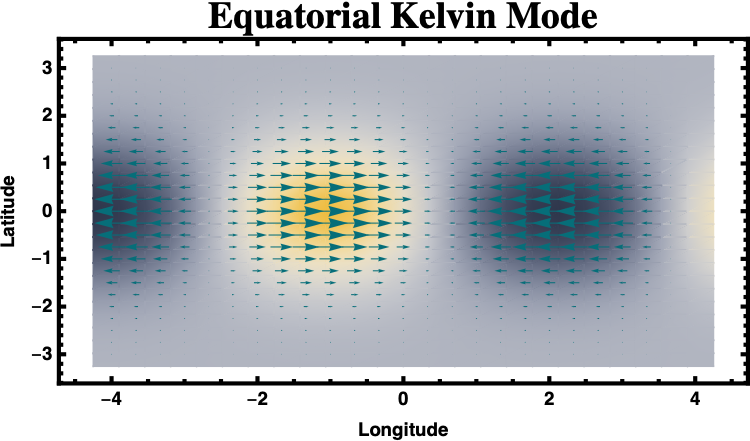
\includegraphics[width = .7 \textwidth]{figs/GD/KelvinWave.png}
\caption{}
\end{figure}

As expected the wave has no meridional velocity and it is symmetric
around the equator.

\subsection{Rossby equatorial waves}\label{rossby-equatorial-waves}

The solution with \(v\) different from zero can now be obtained by
transforming the equation into a single equation for \(v\)

\[\frac{\partial^{2} v}{\partial y^{2}} + \left[ (\omega^2 - k^2) -\frac{k}{\omega} - y^2\right] v = 0\]

note that this equation has been obtained assuming \(k^2 \neq \omega^2\)
so it does not contain the Kelvin waves, as expected. The equation a
classical equation of the Sturm-Liouville type and it has solutions
found in the XIX century in terms of Hermite polynomials weighted by a
gaussian centered at the equator. These solution exist only if the
following condition is satisfied

\[\omega^2 - k^2 -\frac{k}{\omega} = 2 n + 1, \qquad  n=0,1,2\cdots\]

that plays the role of a dispersion relation. Fig. \texttt{fig:72} shows
the dispersion diagram. For every integer n there three possible
solutions, two are high frequency inertia-gravty waves, one traveling
west and one traveling east and a single westward moving wave. The case
\(n=0\) is special is a wave where both gravity and rotation are
important and it behave lie a Rossby wave for large negative wavenmbers
and as a gravity wave for larger positive wavenumbers. These mixed waves
can then be found both traveling east or west.

\begin{figure}
\centering
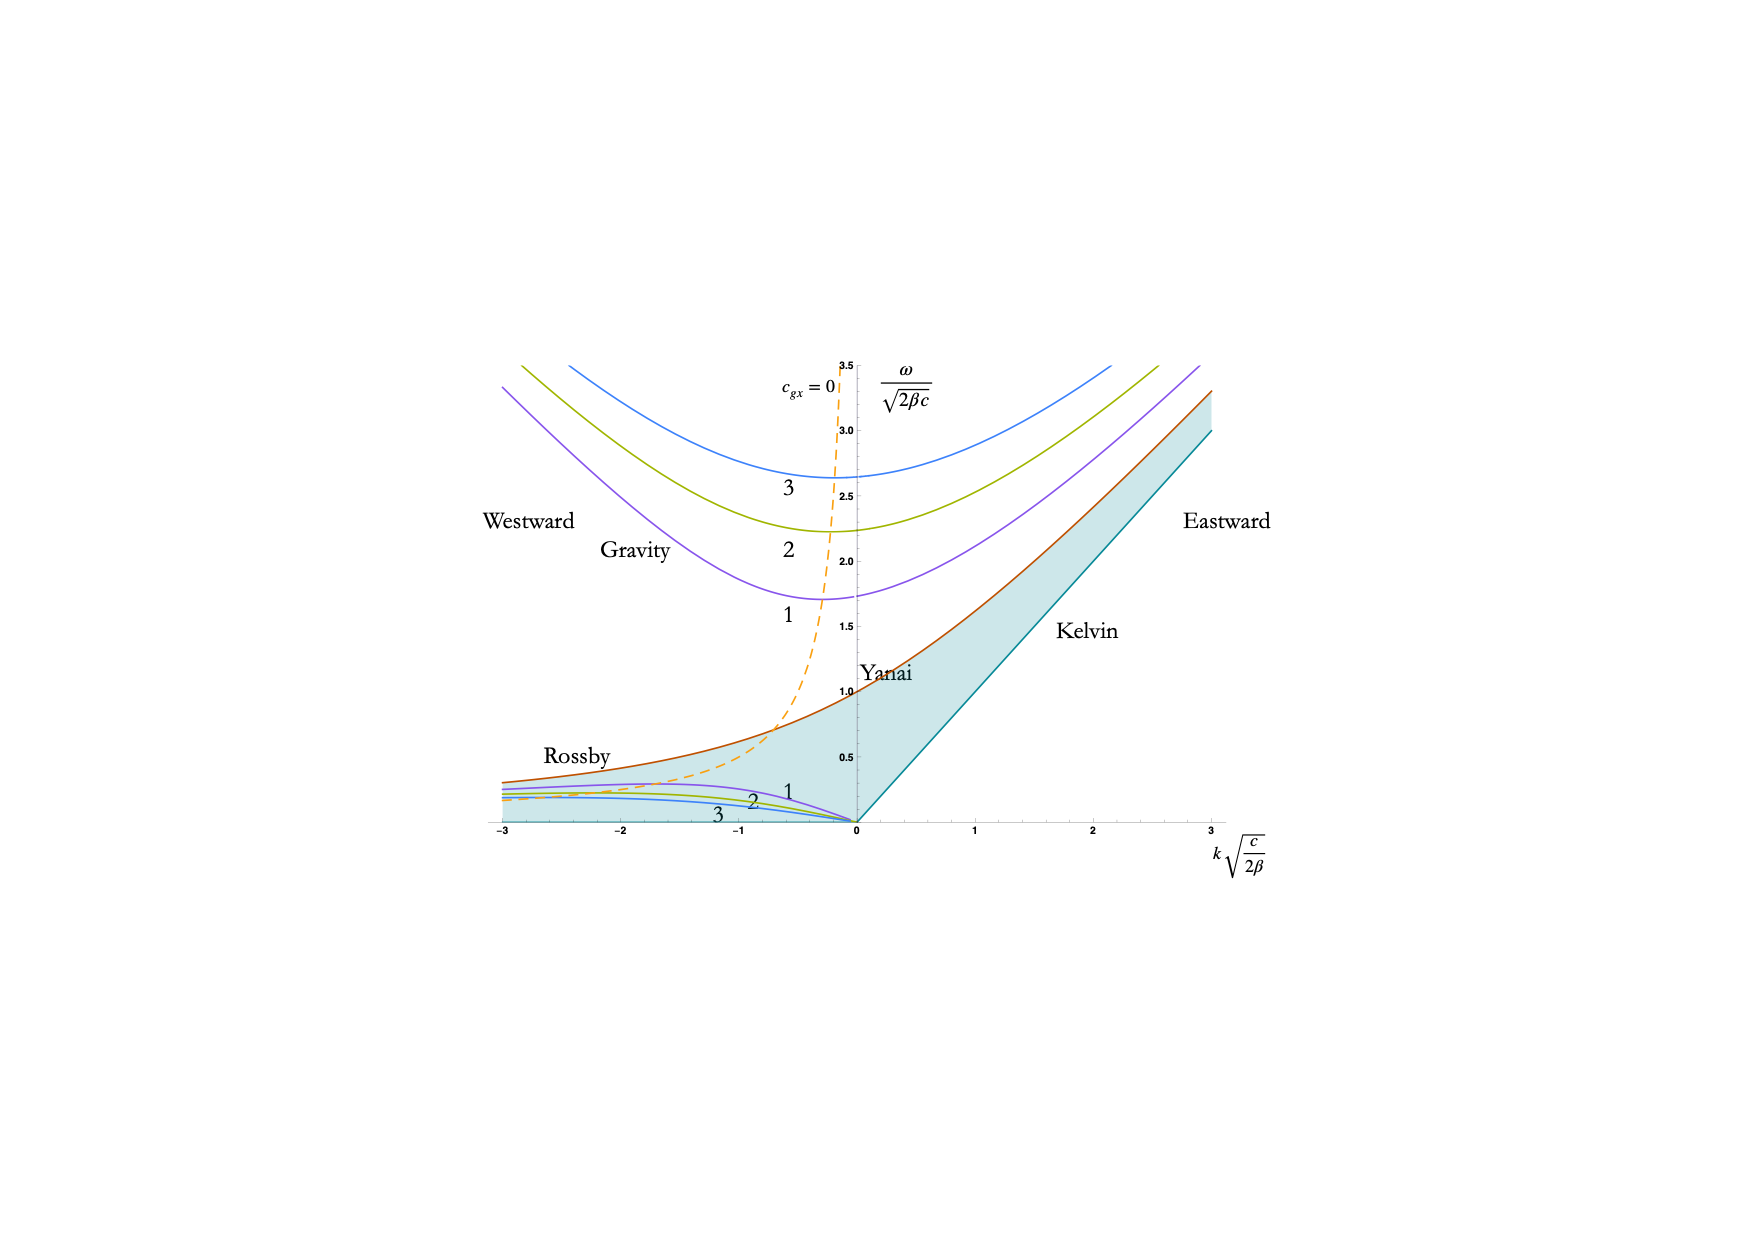
\includegraphics[width = .7 \textwidth]{figs/GD/TropDisp.png}
\caption{Dispersion relation for tropical Waves.}
\end{figure}

The longitudinal group velocity can be found from
eq.(\texttt{eq:tropdisp}) using the rules for the differentiation of
implicit functions (see Appendix \texttt{chp:B} we get

\[c_{gx} = \frac{\partial \omega}{\partial k} = \frac{2 k \omega +1}{2\omega^2 + k/\omega}\]

the line of zero group speed is the limit between west and east
propagation of energy. The Kelvin waves always move erngy eastward,
where the Rossby mode can transfer energy either west or east, depending
on wavelength.

Since the solution to eq. (\texttt{eq:tropdisp}) can be written as

\[v(x,y,t) = H_n(y)\exp{(-\frac{1}{2}y^2)} \cos( k x - \omega t)\]

we can then obtain also the solutions for the zonal velocity and the
height

\[\begin{aligned}
u &= \frac{\exp(-y^2/2)}{\omega^2 -k^2}[ -2 k n H_{n-1}(y) \sin( k x - \omega t) + y k H_n(y) \sin( k x - \omega t) + \\
&y \omega H_{n}(y) \sin( k x - \omega t) ] \\
\phi &= \frac{\exp(-y^2/2)}{\omega^2 -k^2} [-2 n \omega H_{n-1}(y) \sin( k x - \omega t) + y k H_n(y) \sin( k x - \omega t) + \\
&y \omega H_{n}(y) \sin( k x - \omega t)]
\end{aligned}\]

\begin{figure}
\centering
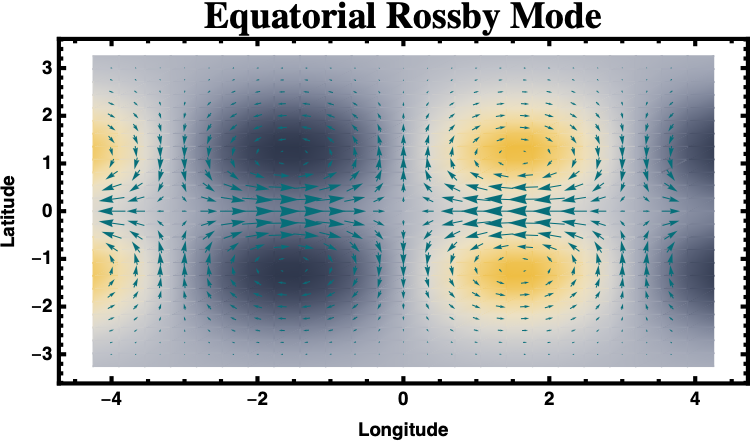
\includegraphics[width = .7 \textwidth]{figs/GD/RossbyWave.png}
\caption{}
\end{figure}

The Rossby mode is in geostrophic balance and for odd \(n\) is symmetric
around the Equator. The divergence/convergence pattern are compensated
mostly by zonal advection, but partially also by meridional motion. The
maximum of the currents are positioned at the Equator, where the maximum
of the geopotential are off equator.

\subsection{Gravity waves}\label{gravity-waves}

Another branch of solution are waves that can be propagate both east or
west under the action of gravity. This are fast traveling waves that
have periods greater than any of the Rossby modes. The flow here is not
in geostrophic balance. Their periods are shorter than a few days for
the first baroclinic mode and about 10 days for the barotropic mode.
Kelvin waves are also fast moving

\begin{figure}
\centering
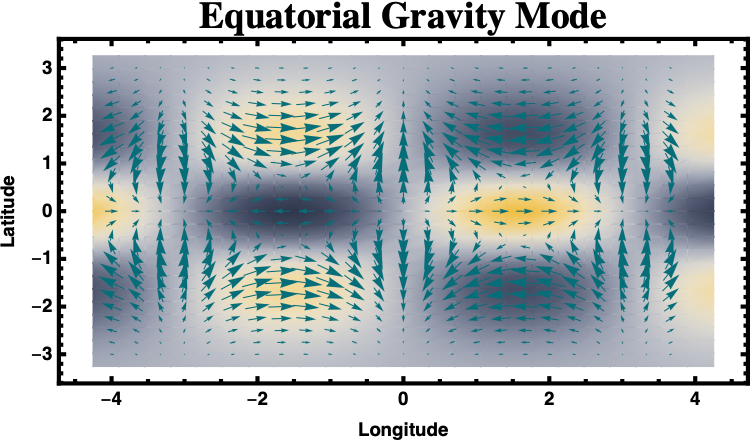
\includegraphics[width = .7 \textwidth]{figs/GD/GravityWave.png}
\caption{}
\end{figure}

\subsection{The Yanai wave}\label{the-yanai-wave}

The Yanai wave is the special oscillation that you get for \(n=0\) in
the meridional dispersion relation. The meridional structure is similar
a kelvin wave since it has the structure of the lowest order Hermite
function, essentially a Gaussian centered at the equator. For westward
propagation and large negative wavenumbers it behaves like a Rossby
wave, whereas for large positive wavenumbers behaves more like a gravity
wave.

Fig. \texttt{fig:75} show the structure of such a wave for the case of
\(k=-1\). The geopotential field is antisymmetric around the equator and
there is considerable cross-equatorial flow. From the pattern of the
flow vorticity is generated right at the Equator.

\begin{figure}
\centering
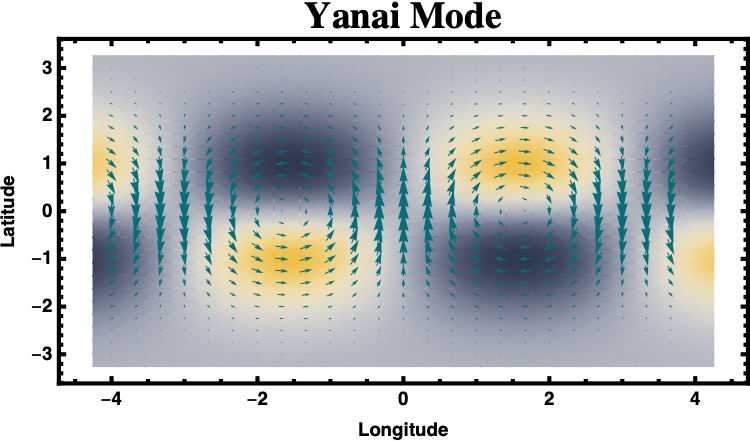
\includegraphics[width = .7 \textwidth]{figs/GD/YanaiWave.png}
\caption{}
\end{figure}

\subsection{Tropical heat sources and forced
motions}\label{tropical-heat-sources-and-forced-motions}

The richness of the dynamics of the tropics is even more important if
one stpo to realize at the over all role that the tropics play in the
general dynamics of the atmosphere and the ocean. Major organized
convection is releasing massive amounts of latent heat energy in to the
tropical atmosphere, the top layers of the ocean store huge amount of
heat that is release through evaporation to feed the same convection.
The latent heat release affects the circulation that in turn though
nonlinear feedback changes the conditions for the convection itself.

It is a non linear problem, usually difficult to investigate and
analyze, but maybe we could get some understanding by using instead the
linear shallow water equations. The richness of the dynamics that we
have seen is suggesting that we may get non trivial results. This was
the approach taken by Gill1980 in the seminal paper on forced motions in
the tropics.

Gill assumed heating sufficiently weak to justify the linear assumption
and he had to eliminate from the equations the fast gravity mode and he
wanted to retain only the Rossby and Yanai modes. Also damping and
cooling was imposed to represent in part the effect of the absent
nonlinear terms. The long time scales jusitfied also the assumption of
stationarity, so the shallow water equations, using the same scales as
before,

\[\begin{aligned}
&\epsilon u - y v = -\frac{\partial \phi}{\partial x}\\
& y u = - \frac{\partial \phi}{\partial y}\\
&\epsilon\phi +\frac{\partial u}{\partial x}+\frac{\partial v}{\partial y} = - Q
\end{aligned}\]

the vertical velocity is then given by

\[w = -\frac{\partial u}{\partial x}-\frac{\partial v}{\partial y} = Q + \epsilon \phi\]

This equations can be combined like before ins single equation for \(v\)

\[\epsilon\frac{\partial^{2} v}{\partial y^{2}} + \frac{\partial v}{\partial x} -\epsilon y^2 v = y \frac{\partial Q}{\partial x} -\epsilon\frac{\partial Q}{\partial y}\]

Then using an expansion on eigenfunctions (i.e. the waves we have found
in the previous section) he was capable of finding the response to a
particular heating distribution. Fig. \texttt{fig:76} show the famous
picture from his paper of the response to a symmetric distribution of
heating centered at the equator. The pressure response, correposngin to
the geopotential field shows a structure typical of a Rossby wave
propagating westward, with two centers on both sides of the Equator,
whereas East of the heating the response is a Kelvin wave propagating
eastward. The corresponding velocity field is such that strong
convergence is ealized at the heating anc cyclonic circulation are
generated north and south. Note that the cyclonic centers are located at
about two length scales from the equator, well outside the equatorial
region.

The vertical velocity balance is particularly interesting. The heating
is almost entirely compensated by vertical motion and we can see that if
had no damping (i.e. \(\epsilon = 0\)) \emph{all} the heating would go
into vertical velocity. However, we should refrain from thinking to get
rid of the heating. In fact the damping terms are crucial to the
existance of this solution, they are part of the physics. Consider Eq
\texttt{eq:gill1} we can see that eliminating the damping will change
the character of the equation and remove all constraint on the
y-structure. In conclusion, damping is an essential component of the
response.

\begin{figure}
\centering
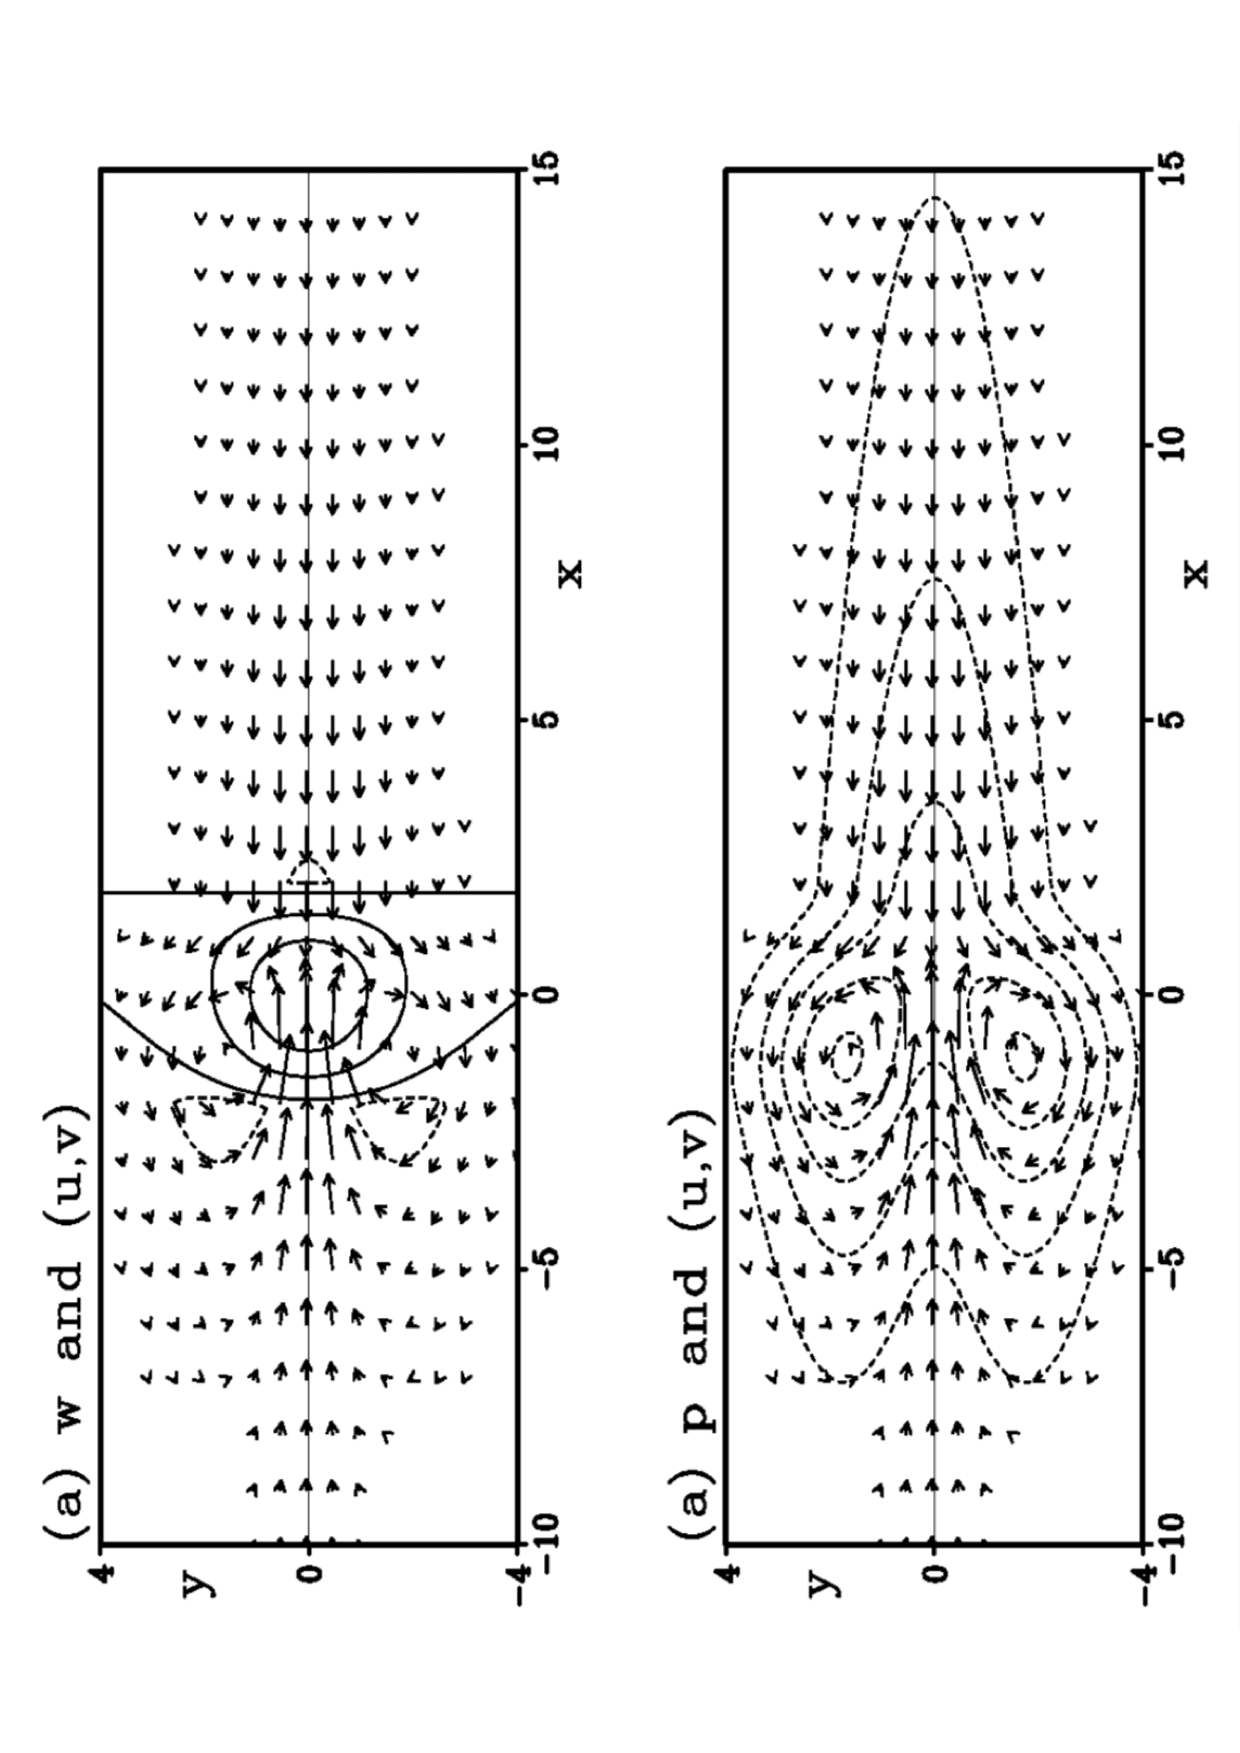
\includegraphics[width = .7 \textwidth]{figs/GD/Gill.png}
\caption{}
\end{figure}

The importance of this discovery was immediately recognized and it is
important to try to expand it to a full tridimensional atmosphere. In a
stratified atmosphere linearize the thermodynamics equation in terms of
the potential temperature around a zonal basic state \(\bar{u}\) in
thermal balance with a temperature distribution \(\bar{\theta}\),

\[\bar{u}\frac{\partial \theta}{\partial x} + v\frac{\partial \bar{\theta}}{\partial z} + w \frac{\partial \bar{\theta}}{\partial z}  = Q\]

% or

\[f \bar{u}\frac{\partial v}{\partial z} - f v\frac{\partial \bar{u}}{\partial z} + w N^2  = Q\]

then if horizontal advection is dominating

\[v \approx \frac{Q H}{f U}\]

but if vertical velocity is the compensating mechanism

\[w \approx Q/N^2, \quad \beta v \approx f \frac{\partial w}{\partial z}\]

so the ratio

\[R =\frac{f^2 U}{\beta N^2H^2}\]

\begin{figure}
\centering
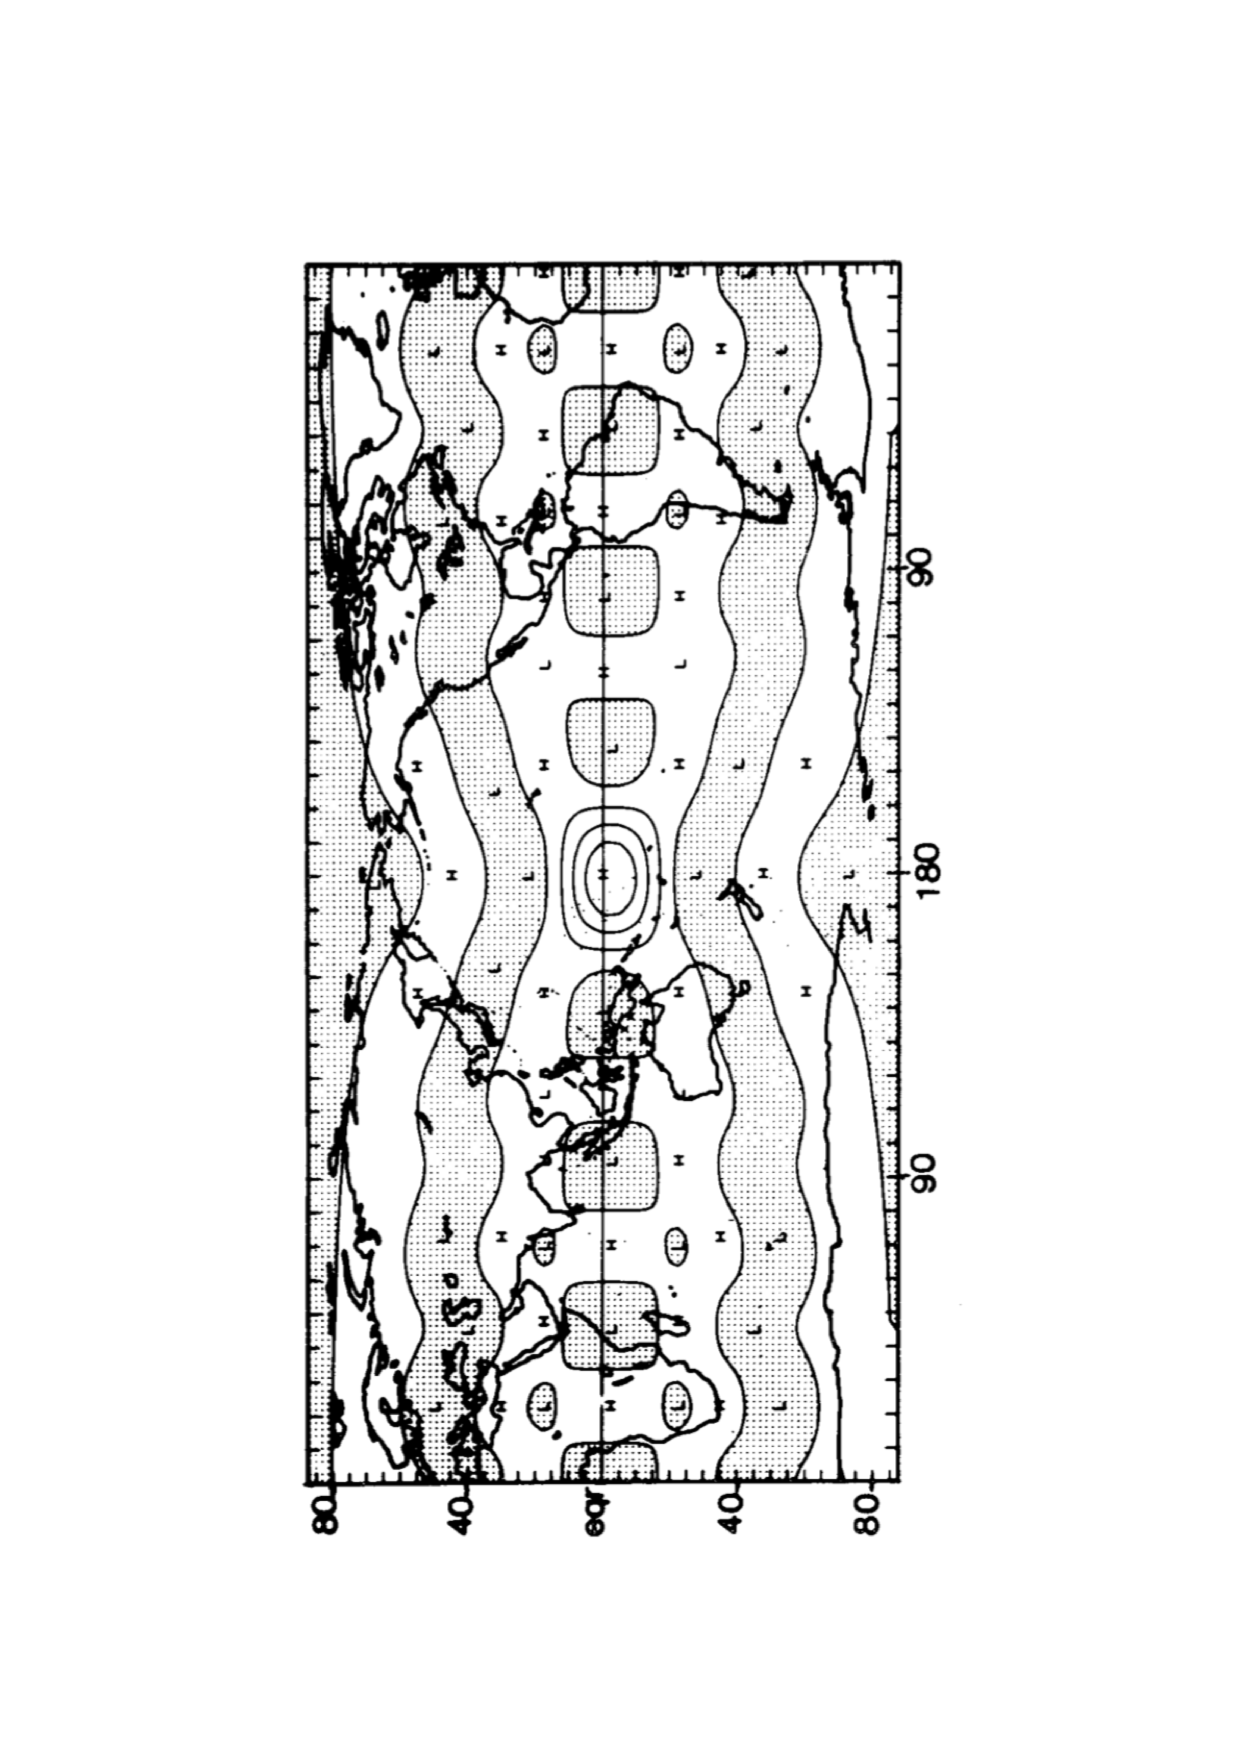
\includegraphics[width = .7 \textwidth]{figs/GD/Heat1.png}
\caption{}
\end{figure}

\begin{figure}
\centering
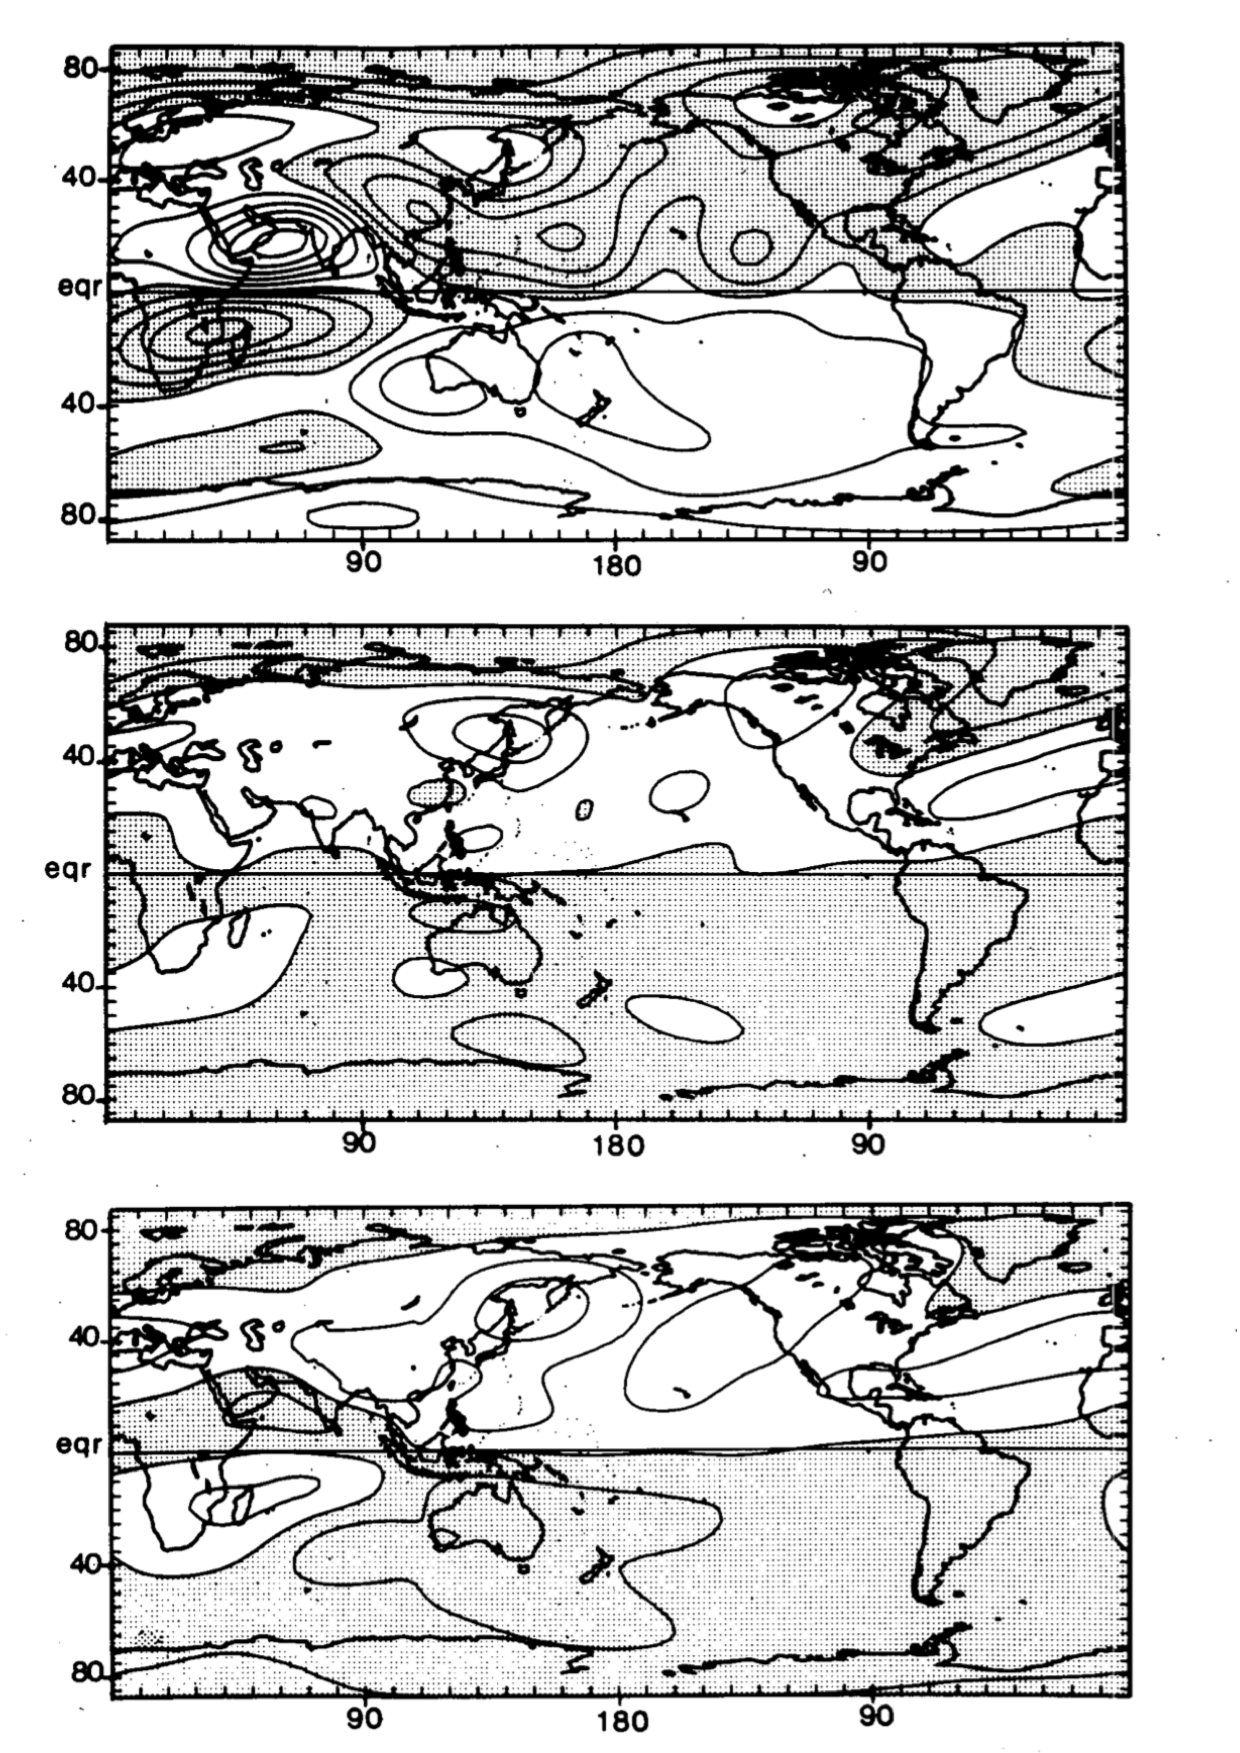
\includegraphics[width = .7 \textwidth]{figs/GD/Heat2.png}
\caption{}
\end{figure}

will tell us which process dominates, assuming that it is the ones
requiring the smallest \(v\). In the tropics R is small, so heating is
compensated by vertical motion, in the mid-latitudes it is th eopposite
and heating is compensated by meridional advection. These ideas were
further put together by Hoskins1981 in more detailed study of the
effects of heating on the global circulation. The basic idea here is the
observation that the cyclonic centres in the Gill local equatorial
response to heating are sufficiently far away from the equator to enter
the area where they can act as vorticity centers for the forcing and
propagation of midlatitude Rossby waves.

The response of an isolated heating source like the one showed in Fig.
:numref\texttt{fig:78} for the upper (200mb), middle (500mb) and lower
(850mb). We see here in the streamfunction clearly the double cyclones
focred by the heating source at the equator and opposite sign vortices
are generated in the lower levels. The upper air cyclones work as
potential vorticity sources and the start a wavetrain of standing
planetary waves that run across the planet.

The thermodynamic picture is completed by Fig. \texttt{fig:79} where we
can see how effective is the compensation by vertical motion of the
heating source. The maximum is at the center of the heating as expected
and it is of course consistent with pattern of divergence and
convergence. We can also see how the alternating areas ofupward and
downward motion extends all around the equator creating significant
effects at very remote locations.

The complete dynamical picture is obtained by looking at the zonal wind
response (Fig. \texttt{fig:80}). We can see clearly the convergence in
the low levels and the divergence in the upper level. The longitudinal
circulation that it is generated in this case is known as the Walker
circulation, fro the name of Sir Gilbert Walker, one of the discoverers
of the Southern Oscillation.

\begin{figure}
\centering
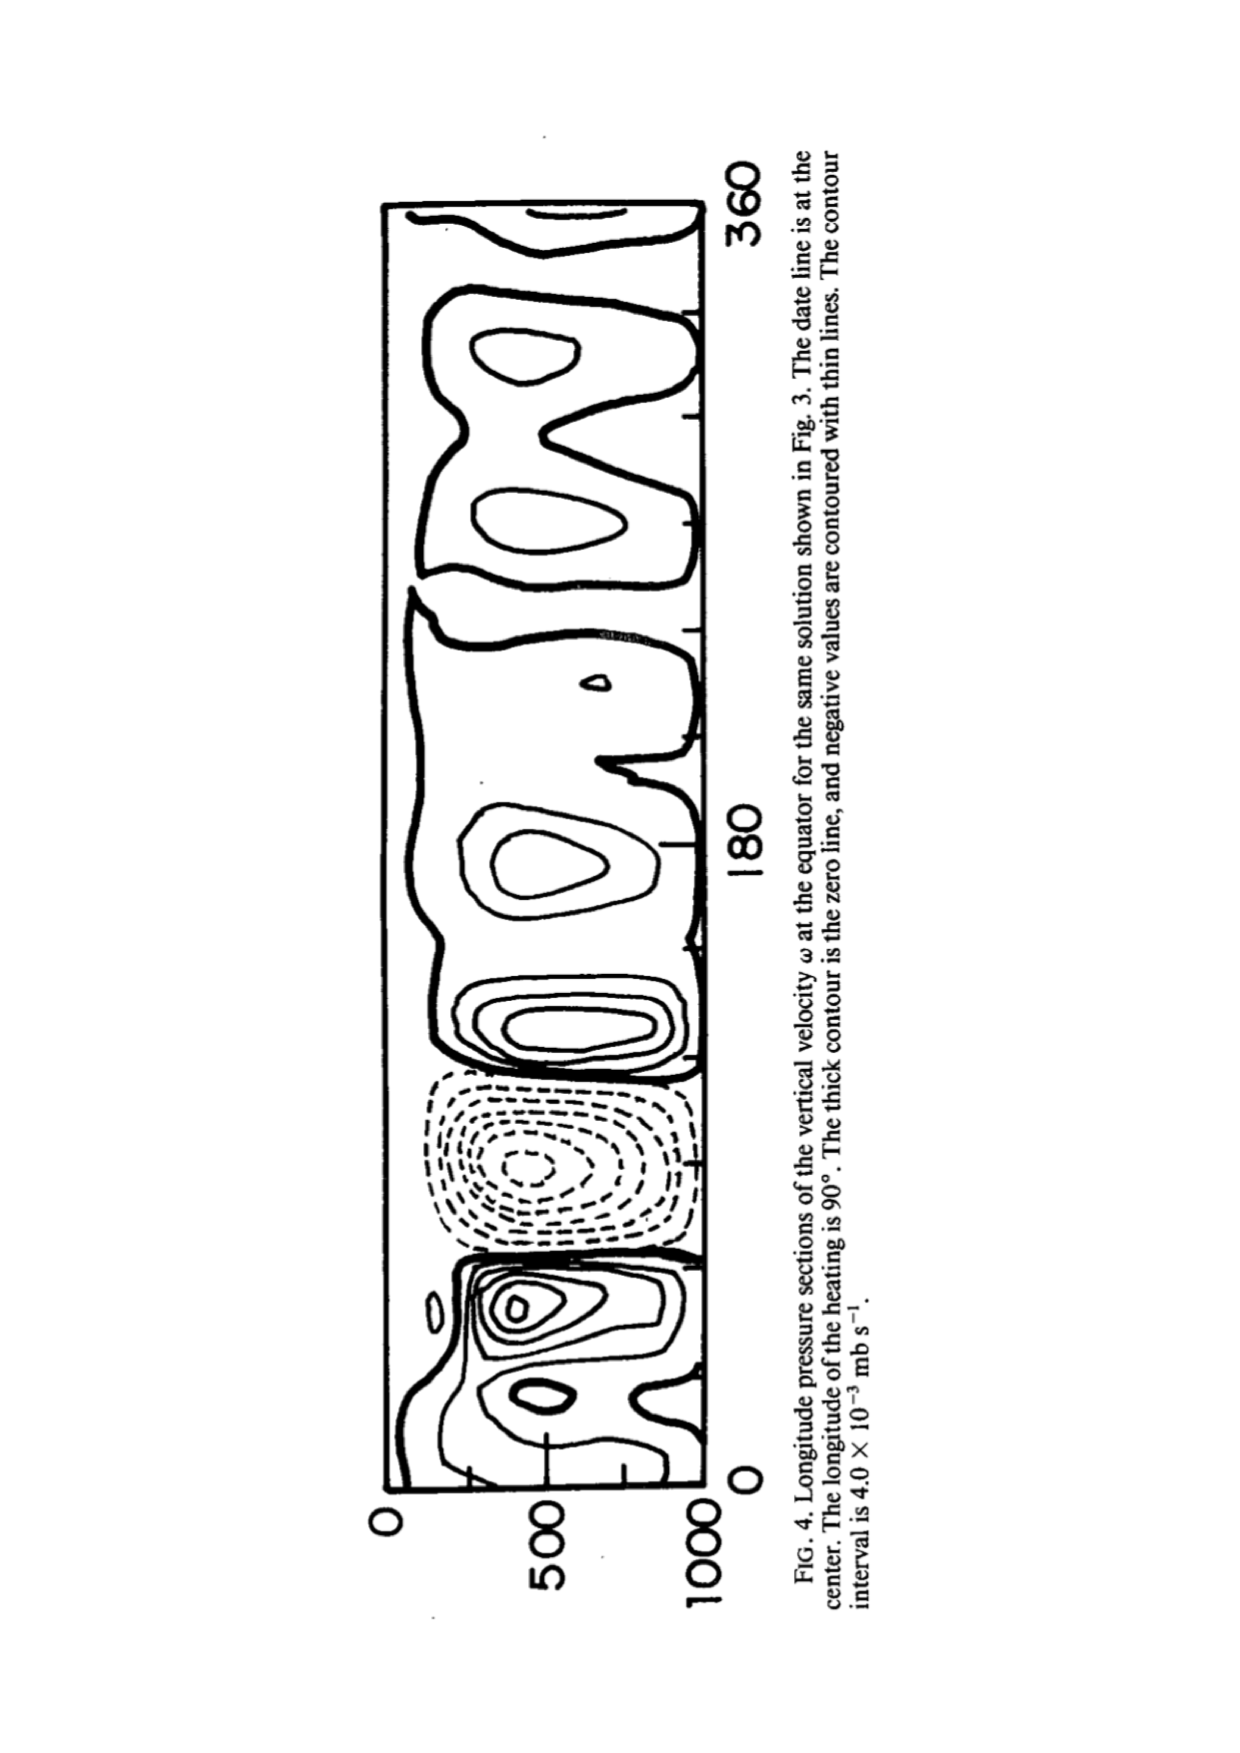
\includegraphics[width = .7 \textwidth]{figs/GD/Heat3.png}
\caption{}
\end{figure}

These investigation have openend the way to the understanding of the
interaction between the ocean and the atmosphere providing physical
basis to the teleconnections that were being discovered almost at the
same time. Evidence of remote effects started emerging in the early
80's, prompted by the investigation of the SST anomalies impact on the
atmospheric circulation. It was unclear until these investigations what
was the mechanism that mediated the impact of the SST on large scale
pattern circulation at planetary scales. Gill and Hoskins work started a
new area of active research and provided a new paradigm to interpret the
interannual variations of climate at planetary scales.

They also are one of the building blocks of more coherent theories of
ocean-atmosphere interactions that were developed in the 90's the working of ENSO mechanism.

\begin{figure}
\centering
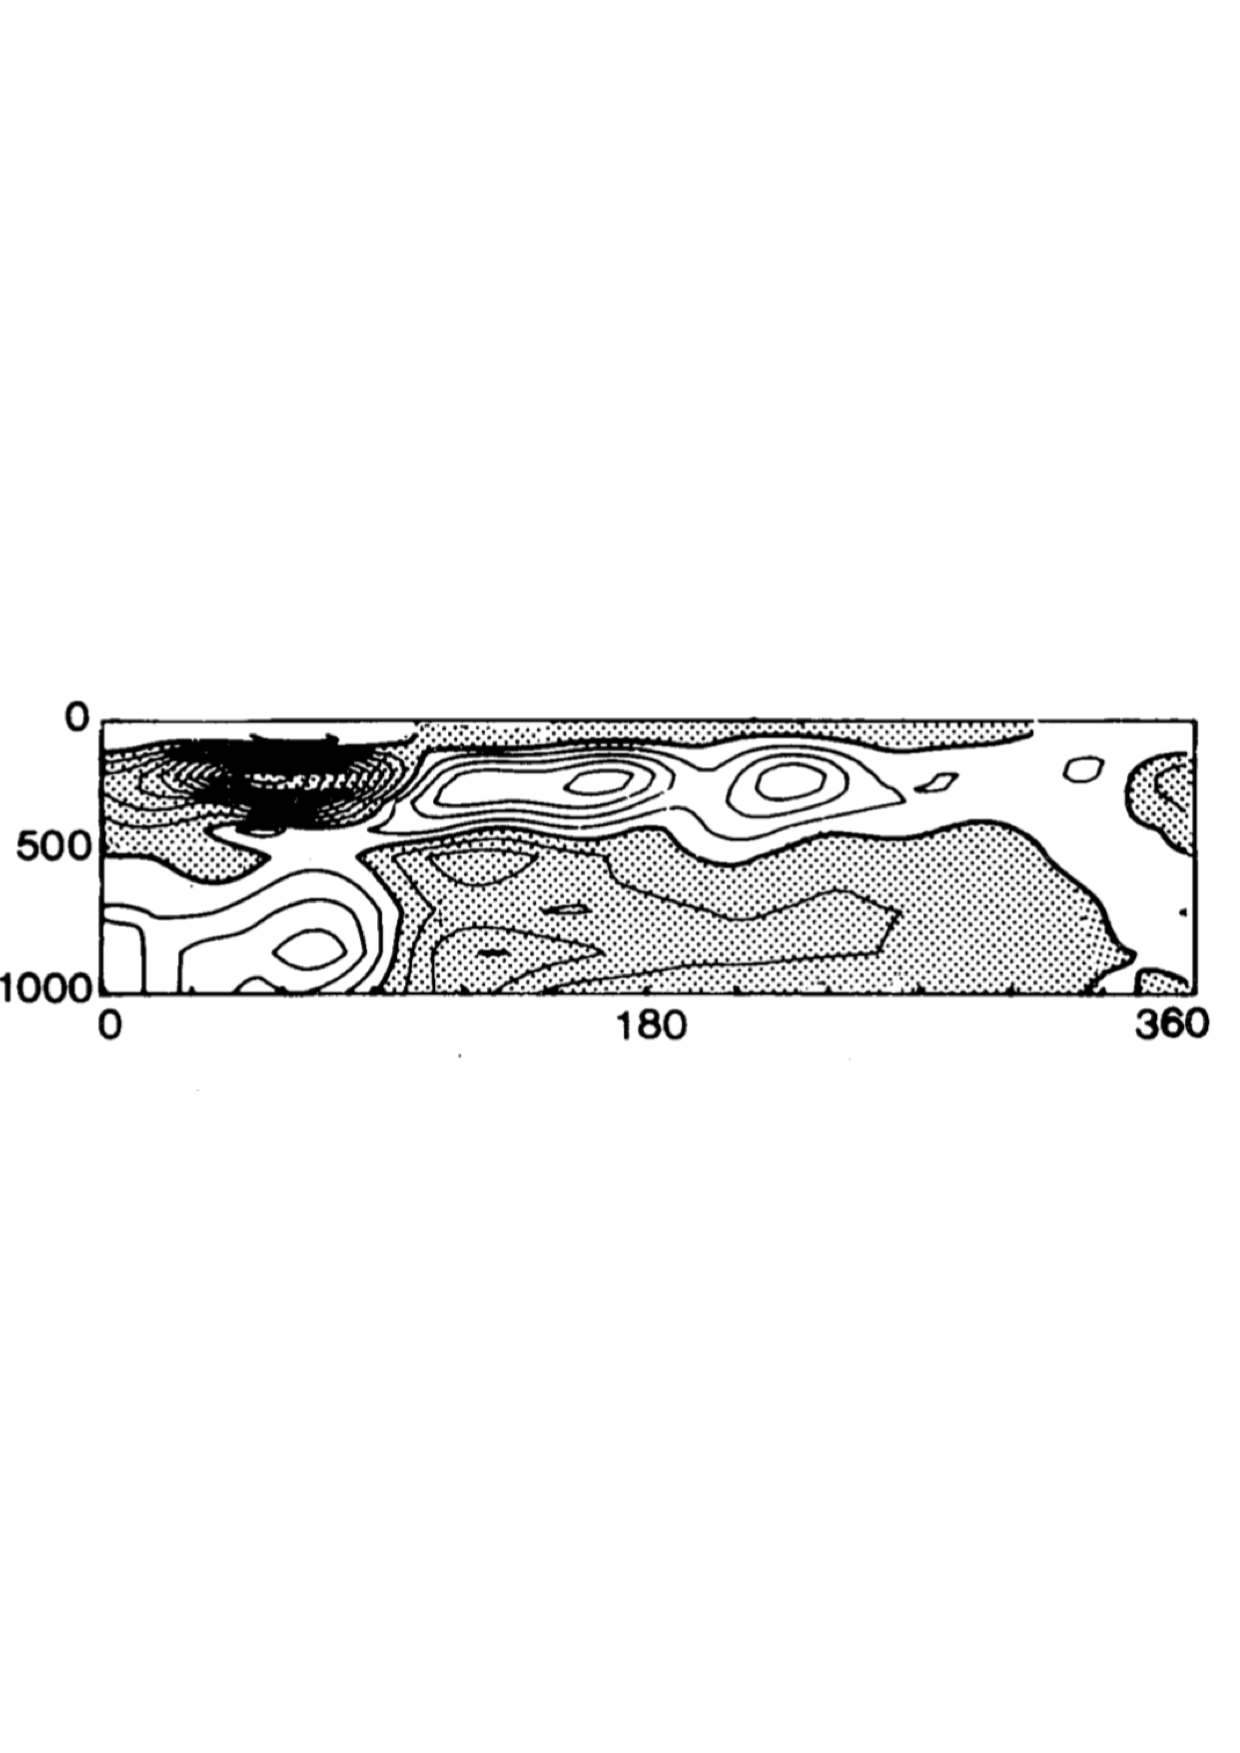
\includegraphics[width = .7 \textwidth]{figs/GD/Heat5.png}
\caption{}
\end{figure}
